\documentclass[tikz,border=3mm]{standalone}
\begin{document}

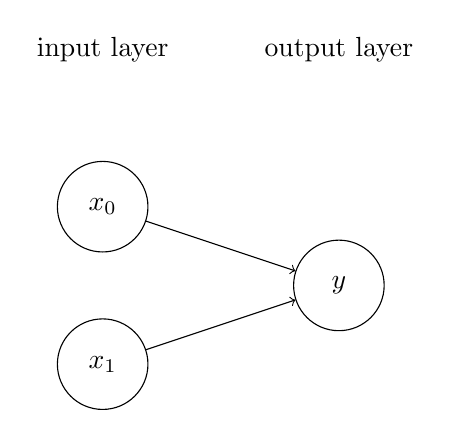
\begin{tikzpicture}
	\tikzstyle{node}=[draw,shape=circle,minimum size=1.15cm]

	\node[node](x0) at (0,2){$x_0$};
	\node[node](x1) at (0,0){$x_1$};
	\node[node](y) at (3,1){$y$};
		
	\draw[->] (x0) -- (y);
	\draw[->] (x1) -- (y);
	
	\draw (0,4) node {input layer};
	\draw (3,4) node {output layer};
\end{tikzpicture}

\end{document}